\chapter{系统架构}
在第\ref{chapter:def}章定义了要解决的问题,并确定了实验的有关假设之后,本章我
来说明分布式二级哈希表的系统架构设计,而在第\ref{chapter:implementation}章中将
详细介绍系统各模块的实现细节。

对于像分布式二级哈希表这样的分布式存储系统,需要解决的关键问题主要包括以下几
点:
\begin{enumerate}
  \item 数据在集群中的单个结点上是如何存储的?
  \item 如何知道集群中哪些服务器结点当前是正常运行的?哪些已经发生了故障无法响
  应?进一步的,如果有结点发生了故障,那么是什么类型的故障?是因为系统负荷过大
  暂时无法响应,还是服务器程序崩溃或者系统故障需要重新启动,亦或是硬盘错误数据
  本地数据无法恢复?
  \item 数据在不同存储节点上是如何分配的?数据是如何存为多个副本的?给定索引如
  何确定数据存放在哪台(些)服务器上?
  \item 如何保证不同副本的数据一致性?
\end{enumerate}
分布式二级哈希表基于一些经典技术,在保证效率的前提下解决了这些问题,如图
\ref{figure:architecture}所示。

\begin{figure}[htb]
  \centering
  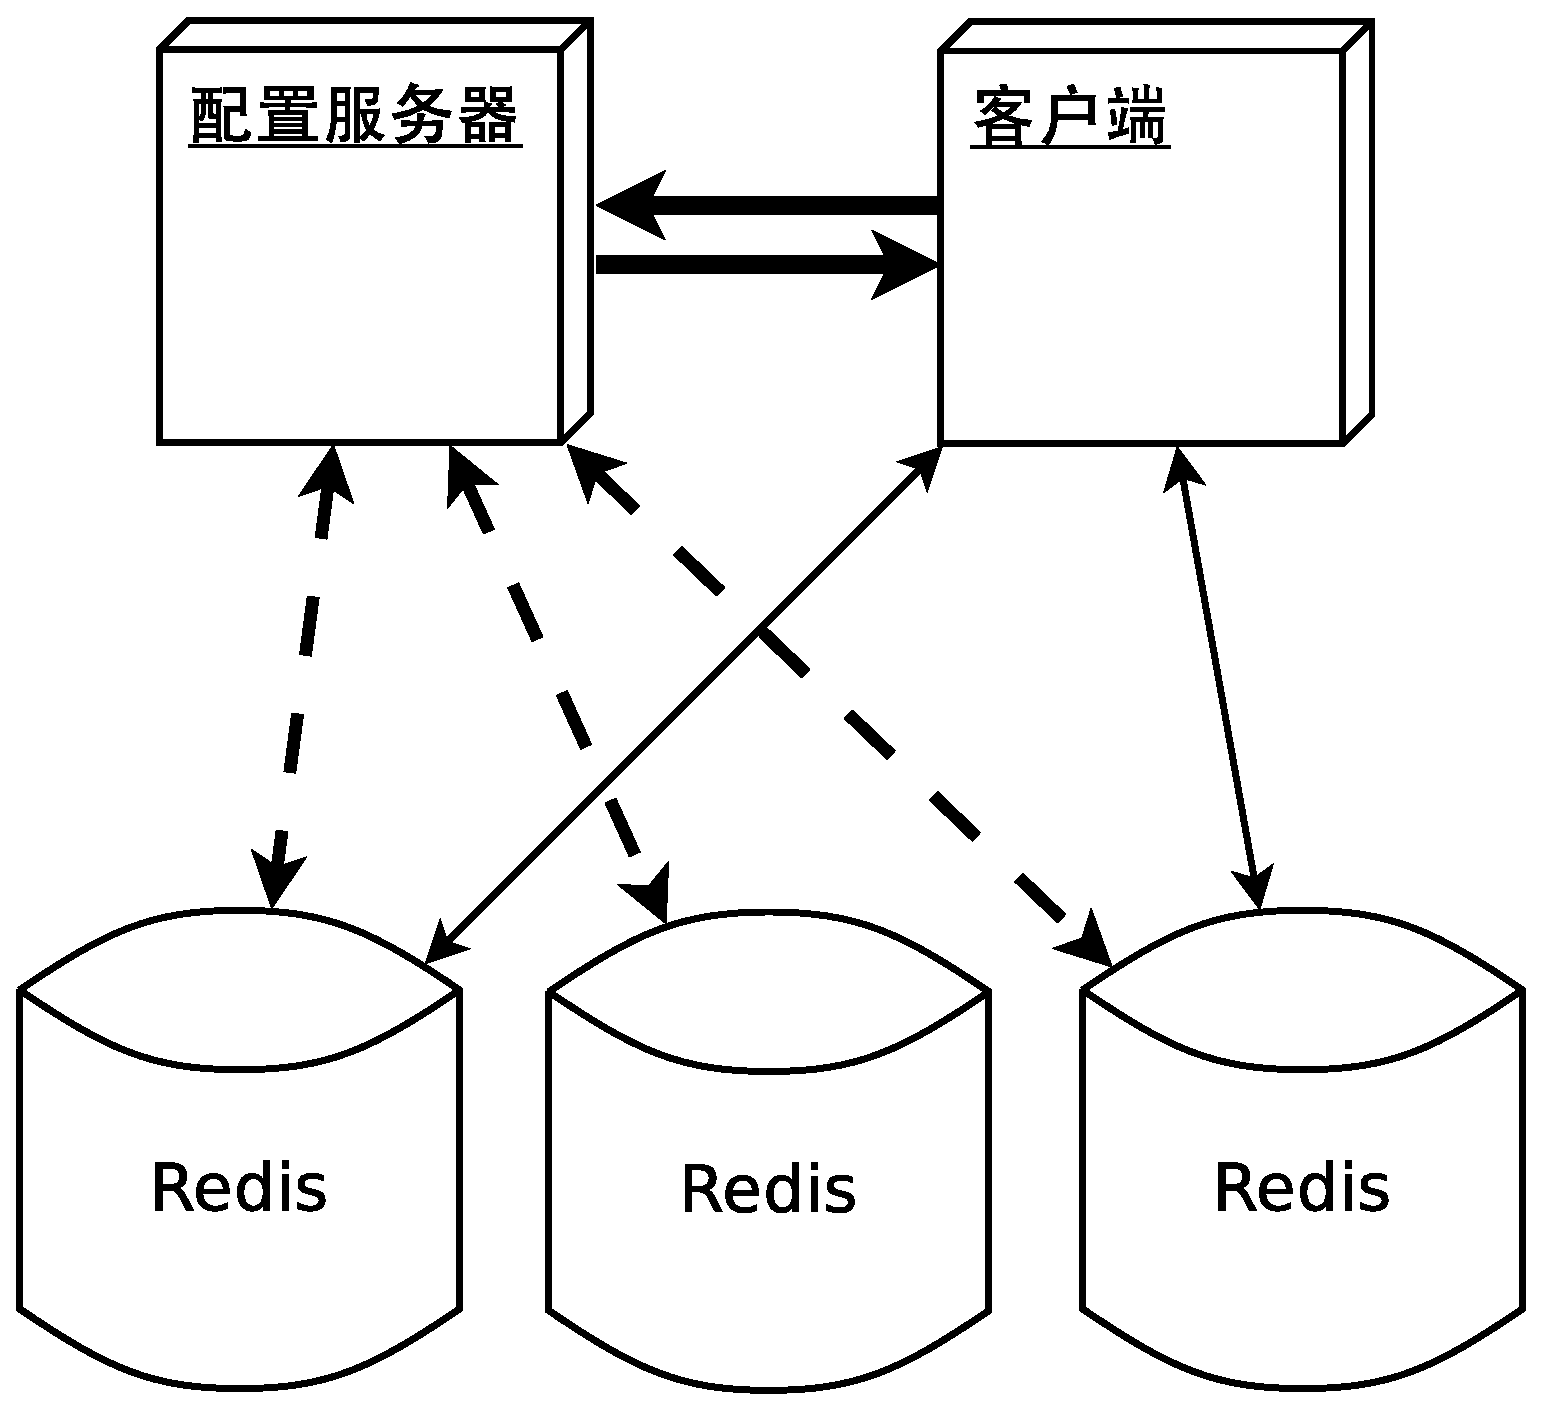
\includegraphics[width=0.8\linewidth]{architecture}
  \caption[分布式二级哈希表系统架构]{分布式二级哈希表系统架构。服务器集群中每
  个存储节点上运行一个Redis服务器进程。集群中设置一台配置服务器,与各节点进行
  心跳通信(虚线箭头),实现一致性哈希。上层应用调用客户端库提供的接口函数,首
  先通过远程过程调用(粗实线箭头)从配置服务器获取某个bucketID对应的一系列存储
  服务器的地址,再遵照协议与这些服务器上的Redis进程进行socket通信(细实线箭头
  ),完成相应操作。}
  \label{figure:architecture}
\end{figure}

在存储服务器集群中的每个结点上,都运行着一个Redis存储服务器进程。Redis是一个开
源本地哈希表项目。与一般的哈希表不同,Redis的值类型除了可以是一般的字符串,还
可以是列表、集合甚至哈希。所以Redis实际上已经解决了本地二级哈希的问题。Redis的
另一个优点是它在应用层实现了一个虚拟存储层,将所有数据存于内存和应用层虚存中大
大提高了系统运行效率。同时,Redis是基于日志的事务型存储系统,保证了操作的原子
性,并具备一定的容错能力。有关Redis的更多细节我将在第\ref{section:redis}节做进
一步介绍。

集群中有一台特殊的配置服务器,通过与集群中其他的存储节点进行心跳通信,来确定当
前有哪些机器在正常运行。当前系统不区分不同的故障类型,一概认为该服务器发生了永
久性错误,之后的操作不再涉及该服务器。由于数据有多份副本,不会发生信息丢失。关
于故障处理的更多细节参见第\ref{section:fault}节。配置服务器的另一个功能是实现
了一致性哈希,对于某个特定的目标数据,根据它的bucketID,配置服务器负责指定多个
服务器结点存放该数据,并维护该信息,从而实现了数据的分配和备份。在第
\ref{section:consistent}节我将详细介绍一致性哈希算法。

分布式二级哈希表提供了一个客户端库,里面包含第\ref{section:api}节罗列的接口函
数供上层应用调用。当上层应用发起请求时,客户端首先通过远程过程调用
\footnote{http://en.wikipedia.org/wiki/Remote\_procedure\_call}从配置服务器获
取存放着该数据的多台目标服务器的IP地址,然后按照Redis规定的协议,通过socket通
信\footnote{http://en.wikipedia.org/wiki/Computer\_network\_programming}同时向
这些目标服务器发起请求并接收应答。为了提高系统的运行效率,客户端还做了多项优
化,并且通过线程池实现了异步请求,详见第\ref{chapter:implementation}章。
